\documentclass[a4paper,11pt]{article}
\usepackage{graphicx}


\title{High Level Design Document \\ Bin-packing VM Consolidation Algorithm}
\author{Atchutuni Bhavana 13MCMT01 \and Terli Venkatesh 13MCMT55 \and Surineni Sampath Kumar 13MCMT49}


\date{\today}
\begin{document}
\maketitle
\pagebreak
\tableofcontents
\pagebreak 

\section{Introduction}
The purpose of this document is to depict the high level
design and the data flow diagram of bin packing
vm consolidation algorithm project.
\section{Modules in the system}
We have decided to divide the whole project into 3 modules. They are
\begin{enumerate}
\item \textbf{ User Interface }

This module is the main interface to the user and  is responsible for building, editing and updating the GUI.
\item \textbf{ Parser }

This module reads the input from file and initializes PM’s and VM’s as specified in it.
\item \textbf{ PM modifier }

This module is responsible for creating physical machines(PM), adding virtual machines(VM) and doing modifications to them. This is also responsible for consolidation operation.  

\end{enumerate}

\begin{figure}[h]
\centering
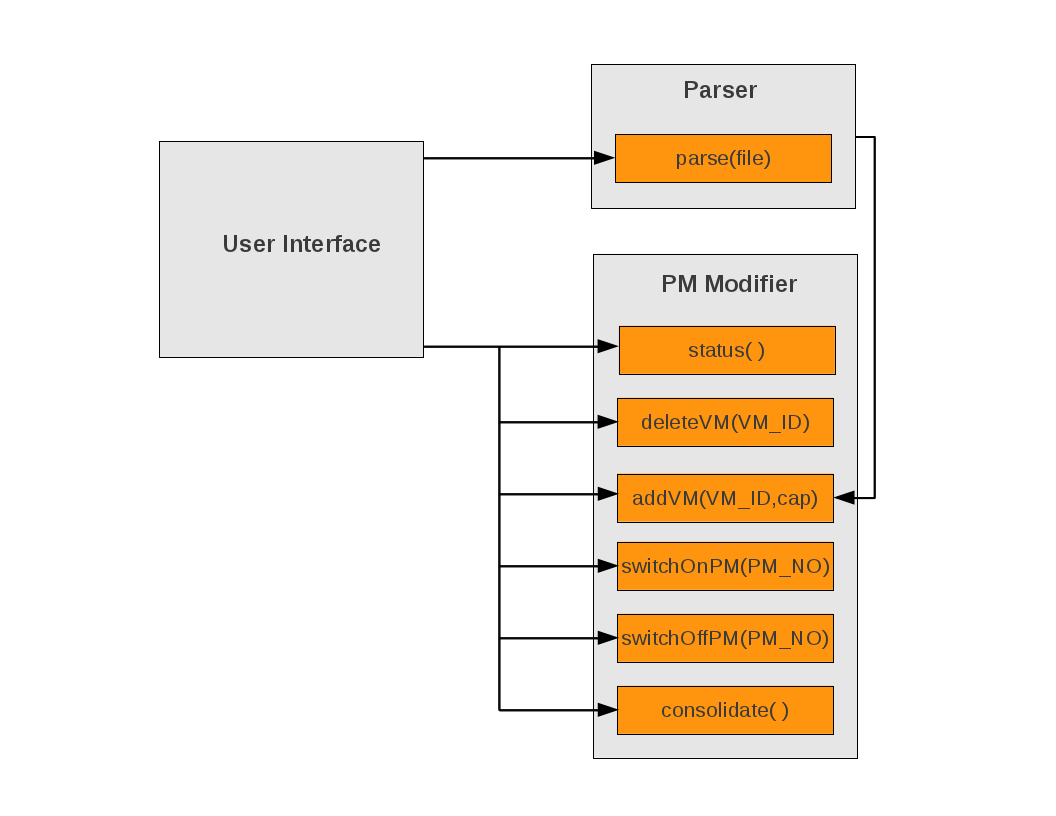
\includegraphics[height=7cm]{images/intrfc.png}
\caption{Interfaces between modules}
\label{fig:interfaces}

\end{figure}

\pagebreak
\subsection{Data flow diagram}

\begin{figure}[h]
\centering
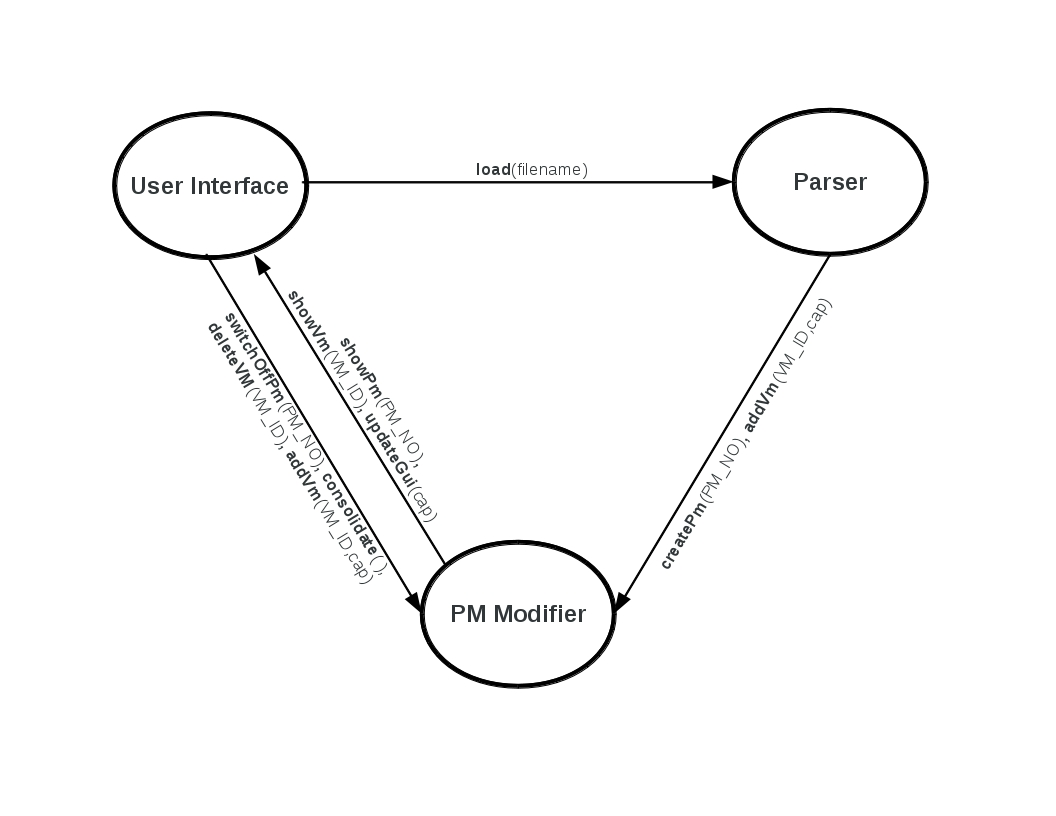
\includegraphics[height=11cm]{images/dfd.jpg}
\caption{Data flow diagram}
\label{fig:modules}

\end{figure}




\subsection{API Specification}
\subsubsection{Modules of the architecture }
\textbf{User Interface Module}
\begin{itemize}
 \item \textbf{Functionality}
 
 The main purpose of this module is to take input from the user and reflect the system state to the user. 
 \begin{figure}[h]
\centering
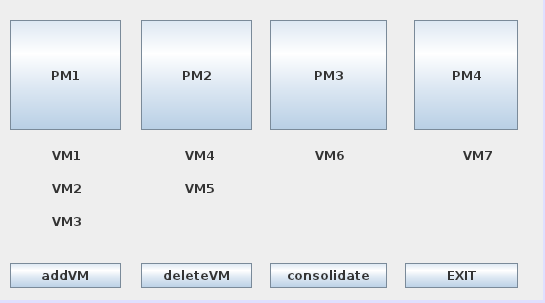
\includegraphics[height=7cm]{images/GUI.png}
\caption{Main user interface}
\label{fig:GUI}

\end{figure}
\end{itemize}
\textbf{Parser}
\begin{itemize}
\item \textbf{Functionality}

The aim of this module is to parse a text file specified by the user, extract the information about PM's and VM's in it.
It then initializes the PM's and adds VM's to them by the help of PM modifier module.

\item \textbf{Interface Description} 

\textbf{parse(filename)}
  
\begin{tabbing}
\hspace*{4cm}\=  \kill
 \textit{Purpose} \> :The purpose of this function is to parse the file specified by the \\ \>user and extract information about PM's and VM's.\\
  \textit{Input Parameter} \> : file path specified by the user \\
  \textit{Output Parameter} \> : VM ID and capacity \\
  \textit{Return Value} \> : If the file is not in the specified format it would return \\ \>\textbf{wrong file format} message \\
  \textit{Called by} \> : User Interface module \\
  \textit{Calls} \> : addVM function of PM modifier
\end{tabbing}
\end{itemize}

\textbf{PM modifier}

\begin{itemize}
\item \textbf{Functionality}

The operations of this module include creating a PM, adding VM's to it, calculating the residual capacity and consolidation.

\item \textbf{Interface Description} 
\\
\textbf{addVM(VM\textunderscore ID, cap)}
  
\begin{tabbing}
\hspace*{4cm}\=  \kill
 \textit{Purpose} \> : The purpose of this function is to add VM's to the PM as \\ \>specified by Parser module and UI module.\\
  \textit{Input Parameters} \> : VM ID and VM capacity. \\
  \textit{Output Parameter} \> : none \\
  \textit{Return Value} \> : If there is no enough space to add VM to a PM it outputs \\ \>\textbf{No enough space} message\\
  \textit{Called by} \> : Parser module and UI module\\
  \textit{Calls} \> : NONE.
\end{tabbing}

\textbf{deleteVM(VM\textunderscore ID)}
  
\begin{tabbing}
\hspace*{4cm}\=  \kill
 \textit{Purpose} \> : The purpose of this function is to delete a VM specified by the user.\\
  \textit{Input Parameters} \> : VM ID. \\
  \textit{Output Parameter} \> : none \\
 \textit{Called by} \> : User Interface module \\
  \textit{Calls} \> : none.
\end{tabbing}

\textbf{switchOffPM(PM\textunderscore NO)}
  
\begin{tabbing}
\hspace*{4cm}\=  \kill
 \textit{Purpose} \> : The purpose of this function is to switch off a PM specified by user.\\
  \textit{Input Parameters} \> : PM number. \\
  \textit{Output Parameter} \> : none \\
  \textit{Return Value} \> : Returns \textbf{It is not possible to switch off}\\ \> \textbf{this PM at this time} if switching off was not successful. \\
  \textit{Called by} \> : User Interface module \\
  \textit{Calls} \> : none.
\end{tabbing}

\textbf{switchOnPM(PM\textunderscore NO)}
  
\begin{tabbing}
\hspace*{4cm}\=  \kill
 \textit{Purpose} \> : The purpose of this function is to switch on a PM specified by user.\\
  \textit{Input Parameters} \> : PM number. \\
  \textit{Output Parameter} \> : none \\
  \textit{Return Value} \> : none \\
  \textit{Called by} \> : User Interface module \\
  \textit{Calls} \> : none.
\end{tabbing}

\textbf{consolidate( )}
  
\begin{tabbing}
\hspace*{4cm}\=  \kill
 \textit{Purpose} \> : The purpose of this function is to run Bin packing algorithm and \\ \> consolidate all the VM's into minimum number of PM's.\\
  \textit{Input Parameters} \> : none \\
  \textit{Output Parameter} \> : none \\
    \textit{Called by} \> : User Interface module \\
  \textit{Calls} \> : none.
\end{tabbing}
\pagebreak
\textbf{status( )}
  
\begin{tabbing}
\hspace*{4cm}\=  \kill
 \textit{Purpose} \> : The purpose of this function is to return the information \\ \>about all the PM's and the VM's in them.\\
  \textit{Input Parameters} \> : none \\
  \textit{Output Parameter} \> : information about the system \\
    \textit{Called by} \> : User Interface module \\
  \textit{Calls} \> : none.
\end{tabbing}
\end{itemize}
\end{document}
